\chapter{Connecteur et schémas}
Le connecteur KF2510 à sept broches est numéroté sur la carte. Utiliser l'orientation de la photographie et les numéros, pas seulement les couleurs des fils. Broche 1 : K30/KL30, alimentation ; 2 : V2 ; 3 : V1 ; 4 : 1WRE, One-Wire ; 5 : KL, K-Line réservée ; 6 : sortie +5 V, 30 mA maximum ; 7 : GND, masse.

Le schéma du voltmètre précise la K-Line réservée et la limite de courant de la sortie +5 V. Les limites générales de tension des entrées analogiques ne sont pas indiquées. Les 12 V mentionnés pour Check Engine ne constituent pas une spécification des autres entrées. Utiliser le schéma adapté au capteur.

Les illustrations originales conservent leurs annotations anglaises ; les fonctions correspondantes sont expliquées dans ce manuel.

\begin{figure}[H]
\centering
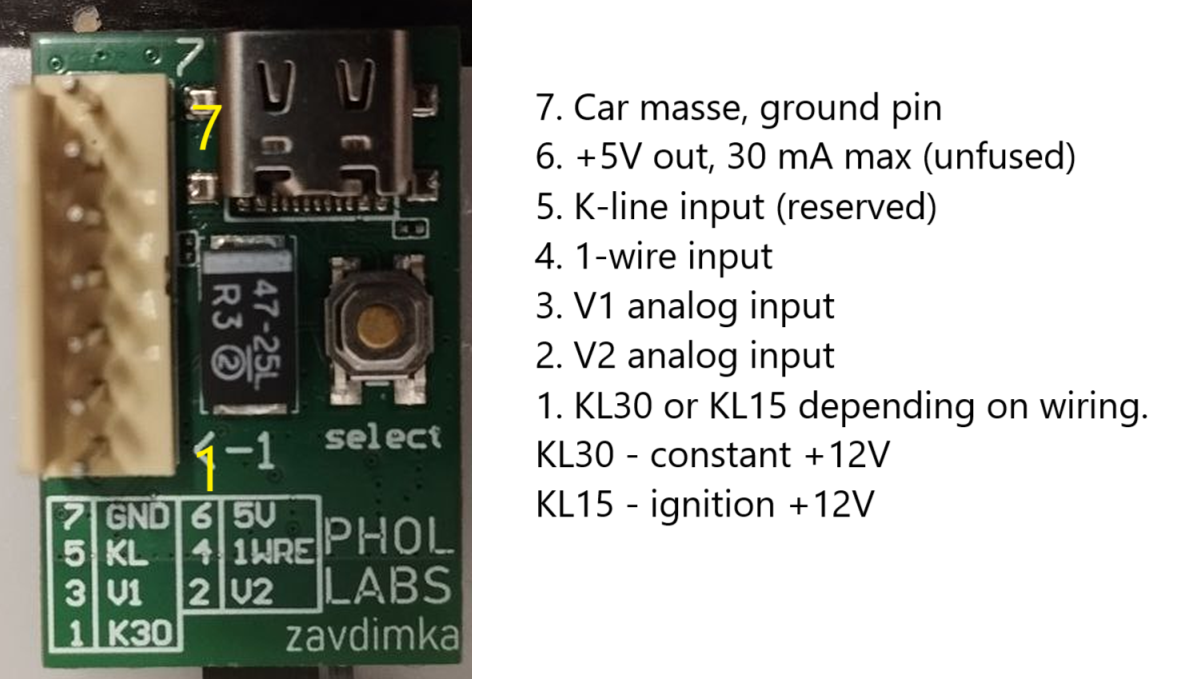
\includegraphics[width=.85\textwidth,height=.60\textheight,keepaspectratio]{figures/ivevo/image20.png}
\caption{Connecteur et schémas}
\end{figure}
\clearpage
\section{Voltmètre}

\begin{figure}[H]
\centering
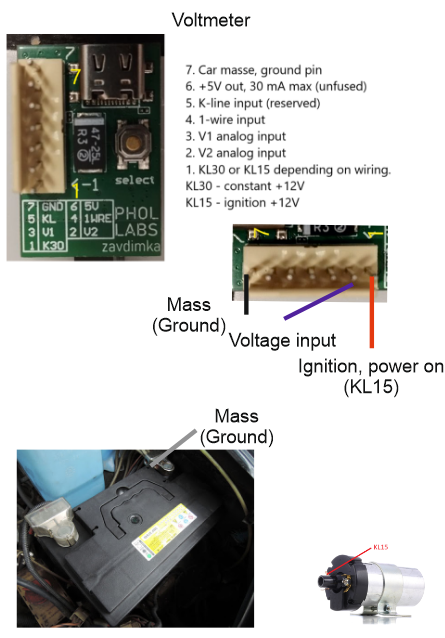
\includegraphics[width=.85\textwidth,height=.60\textheight,keepaspectratio]{figures/ivevo/image5.png}
\caption{Voltmètre}
\end{figure}
\clearpage
\section{Indicateur de rapport}

\begin{figure}[H]
\centering
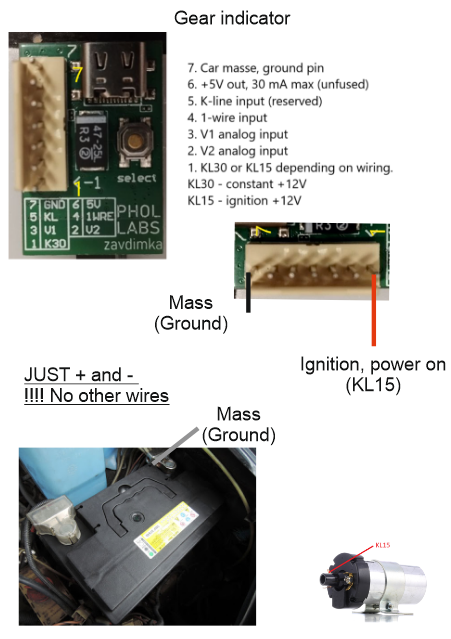
\includegraphics[width=.85\textwidth,height=.60\textheight,keepaspectratio]{figures/ivevo/image6.png}
\caption{Indicateur de rapport}
\end{figure}
\clearpage
\section{Pression d’huile}

\begin{figure}[H]
\centering
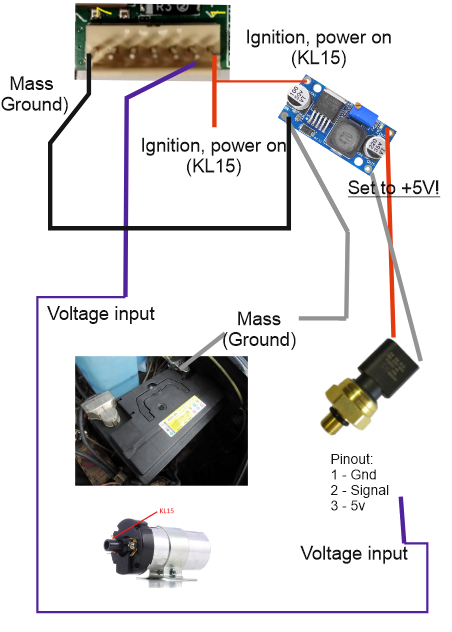
\includegraphics[width=.85\textwidth,height=.60\textheight,keepaspectratio]{figures/ivevo/image1.png}
\caption{Pression d’huile}
\end{figure}
\clearpage
\section{Thermomètre NTC}

\begin{figure}[H]
\centering
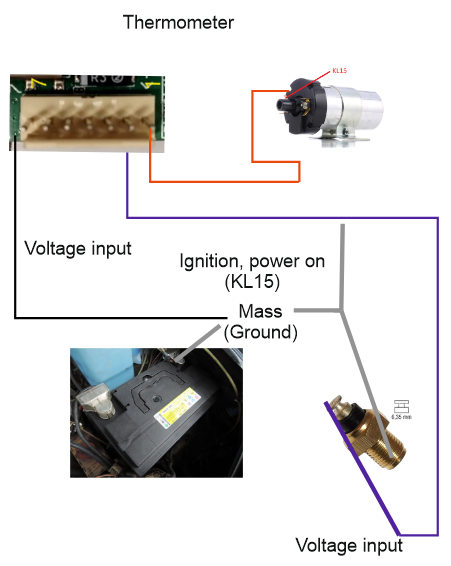
\includegraphics[width=.85\textwidth,height=.60\textheight,keepaspectratio]{figures/ivevo/image13.png}
\caption{Thermomètre NTC}
\end{figure}
\clearpage
\section{Thermomètre numérique}

\begin{figure}[H]
\centering
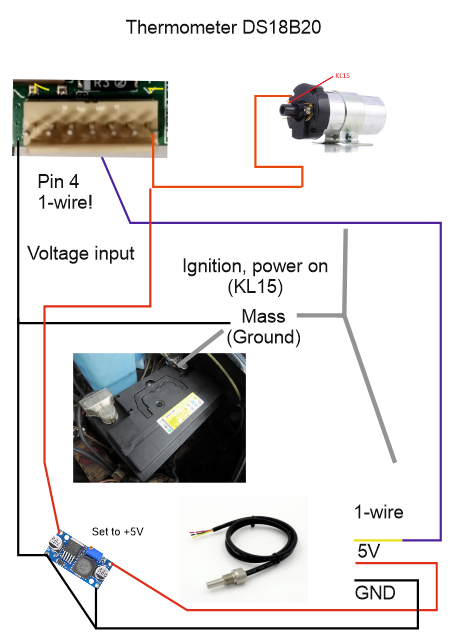
\includegraphics[width=.85\textwidth,height=.60\textheight,keepaspectratio]{figures/ivevo/image8.png}
\caption{Thermomètre numérique}
\end{figure}
\clearpage
\section{Lambda large bande}

\begin{figure}[H]
\centering
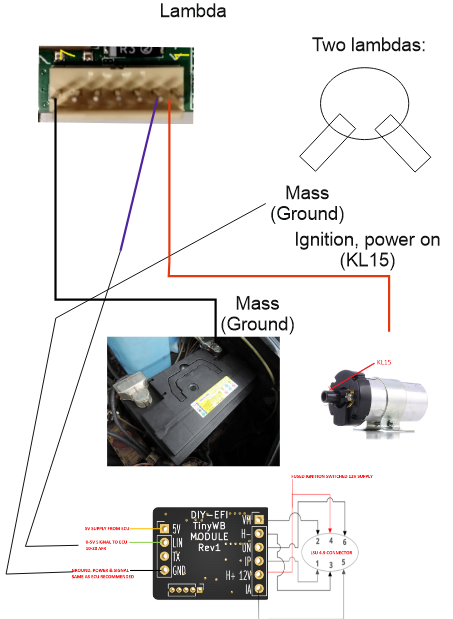
\includegraphics[width=.85\textwidth,height=.60\textheight,keepaspectratio]{figures/ivevo/image3.png}
\caption{Lambda large bande}
\end{figure}
\clearpage
\section{Suralimentation}

\begin{figure}[H]
\centering
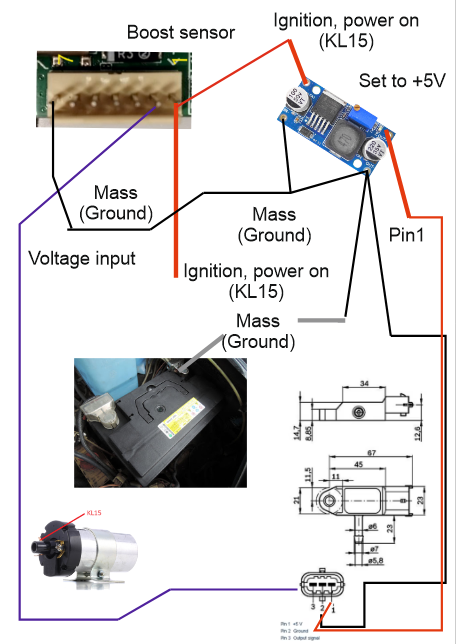
\includegraphics[width=.85\textwidth,height=.60\textheight,keepaspectratio]{figures/ivevo/image17.png}
\caption{Suralimentation}
\end{figure}
